\section{Gerenciamento de \textit{workflows}}

Ferramentas de gerenciamento de \textit{workflows} se mostram importantes no mercado por conferirem escalabilidade ao processo de ETL. Em geral, essas ferramentas representam um \textit{workflow} como um grafo acíclico direcionado~(DAG, do inglês \textit{directed acyclic graph}), onde nós representam transformações e arestas representam a dependência entre os nós.
Nesta seção, consideramos algumas das principais ferramentas de código aberto disponíveis atualmente, a saber: \textit{Oozie}~\cite{ooziewebsite}, \textit{Aurora}~\cite{aurorawebsite}, \textit{Luigi}~\cite{luigigit}, \textit{Azkaban}~\cite{azakbanwebsite} e \textit{Airflow}~\cite{airflowwebsite}. Esta análise é feita a partir de critérios de adequação ao contexto do TRE-RN, detalhados a seguir.

% e fazemos uma análise em todas usando critérios de usabilidade no mercado, principal propósito da ferramenta, dependência de outras ferramentas, experiência usuário(UX do inglês \textit{user experience}), overhead de criação dos jobs, linguagem de programação usada, arquitetura da ferramenta, análise de logs, manutenção da ferramenta, configuração do ambiente e documentação e exemplos. As ferramentas que analisamos são: .
%- usabilidade no mercado
%- principal propósito da ferramenta
%- dependência de outras ferramentas
%- exeperiência usuário
% - overhead de criação dos jobs
%- linguagem de programação usada
%- arquitetura da ferramenta
%- análise de logs
%- manutenção da ferramenta
%- configuração do ambiente
%- documentação e exemplos

\subsection{Critérios de adequação}

Os principais desafios enfrentados pelo TRE-RN em relação a seu processo de gerenciamento de \textit{workflows} de ETL envolvem (i)~o monitoramento do número crescente de \textit{workflows}; (ii)~a análise de \textit{logs} de execução, em caso de eventuais erros, e; (iii)~a dificuldade de alteração de um \textit{workflow} existente. Os critérios detalhados abaixo foram escolhidos por uma questão de viabilidade ou por ajudarem a mitigar pelo menos um desses desafios. 

\textbf{Adequação à infraestrutura} - a ferramenta deve contemplar a infraestrutura do TRE-RN, onde o processo de ETL é realizado a partir de um único servidor. Assim, ferramentas propostas para infraestruturas distribuídas devem ser descartadas.  

\textbf{Disseminação e suporte} - a ferramenta deve ter uma ampla comunidade de usuários que endossem seu uso, particularmente grandes empresas de TI. Além disso, a comunidade de usuários deve ser ativa no suporte à resolução de problemas encontrados no uso cotidiano da ferramenta.

\textbf{Documentação} - a ferramenta deve ser bem documentada e oferecer um bom número de exemplos de uso, facilitando assim o aprendizado por parte dos servidores.
% Para que os servidores consigam usar com facilidade, precisamos que a ferramenta tenha uma documentação bastante rica e com vários exemplos, com isso o processo de desenvolvimento fica mais rápido, como também o processo de debug.

\textbf{Interface gráfica} - a ferramenta deve apresentar uma interface gráfica interativa e intuitiva, evitando o uso de linha de comando. 

\textbf{Criação de \textit{workflows}} - a ferramenta deve simplificar este processo.
A linguagem Python deve ser preferencialmente adotada, por já ser utilizada em parte do ETL existente.

% Devido a pouca quantidade de pessoas e alta demanda pela seção que será responsável pela manutenção da ferramenta, a criação dos jobs devem ser simples de serem desenvolvidos e mantidos. 
% Além disso, existe uma preferência de que os jobs sejam desenvolvidos em alguma linguagem de programação conhecido pelos servidores,  preferencialmente Python, por também haver parte do ETL existente feito em python. Com isso,  não será necessário um aprendizado extra para o uso da ferramenta,

\textbf{Agendamento} - a ferramenta deve possuir um agendador de execução próprio, evitando assim a dependência em relação ao CRON.
% a necessidade de se usar duas ferramentas e centralizando tudo em apenas um único local, facilitando o processo de manutenção e gerenciamento.

\textbf{\textit{Logs} de execução} - a ferramenta deve otimizar o processo de depuração de erros.
% Apesar de não ser recorrente, erros acontecem nos jobs funcionando atualmente. A forma como fazemos atualmente para encontrar estes erros é extremamente precária e demanda muito tempo. Com isso em mente, é necessário que a ferramenta possa mostrar os logs das transformações para que o processo de debug seja mais rápido e eficiente, prevenindo que erros perdurem por muito tempo.

% \begin{figure}[!t]
%     \centering
%     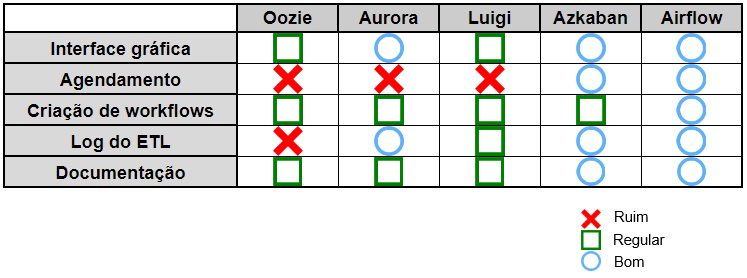
\includegraphics[width=\linewidth]{Imagens/Solucao}
%     \caption{Comparativo ferramentas}
%     \label{fig:comparativo}
% \end{figure}

\begin{table}
\caption{Comparativo entre ferramentas de gerenciamento de \textit{workflow} segundo critérios de adequação ao TRE-RN.}\label{tab:comparativo}
\scalebox{0.8}{
\begin{tabular}{ r|c|c|c|c|c } 
\hline
  & \it{Oozie} & \it{Aurora} & \it{Luigi} & \it{Azkaban} & \it{Airflow}\\
\hline
Infraestrutura & \xmark & \xmark & \cmark & \cmark & \cmark \\
\hline
Suporte & --- & --- & \cmark & \cmark & \cmark \\ 
\hline
Documentação & --- & --- & Regular & Regular & Bom \\ 
\hline
Interface & --- & --- & Regular & Bom & Bom \\ 
\hline
Criação & --- & --- & Regular & Regular & Bom \\ 
\hline
Agendamento & --- & --- & Ruim & Bom & Bom \\ 
\hline
\it{Logs} & --- & --- & Regular & Bom & Bom \\ 
\hline
\end{tabular}
}
\end{table}

\subsection{Análise das ferramentas}

Um resumo da avaliação das principais ferramentas de gerenciamento de \textit{workflows} a partir dos critérios acima pode ser visto na Tabela~\ref{tab:comparativo}. A seguir, discutimos individualmente cada ferramenta apresentada. As ferramentas \textit{Oozie}~\cite{ooziewebsite} e \textit{Aurora}~\cite{aurorawebsite} foram descartadas \textit{a priori} desta análise por dependerem de infraestruturas distribuídas.

% \subsection{Oozie}

% O Oozie é um gerenciador de workflow desenvolvido pela ASF para agendamento de tarefas Hadoop~\cite{}. Apesar desta dependência da infraestrutura Hadoop, possui uma comunidade ativa para desenvolvimento e suporte, por ter sido lançado há muito tempo no mercado. Além disso, possui uma documentação muito bem estruturada e completa para quem deseja usar a ferramenta.

% O Oozie não possuir interface gráfica nativa, dependendo de ferramentas externas como HUE~\cite{} ou Eclipse~\cite{}. A Figura~\ref{fig:hue} mostra a visualização de um workflow usando a ferramenta HUE. Também é possível visualizar \textit{logs} de execução de \textit{jobs}, ou acessá-los por linha de comando.

% Na modelagem do Oozie, um \textit{job} é um grafo acíclico direcionado (DAG, do inglês \textit{directed acyclic graph}), criado usando a \textit{Hadoop Process Definition Language}~(hPDL), um formato baseado em XML. É possível criar DAGs visualmente usando ferramentas auxiliares, como os próprios HUE e Eclipse. 
% % No entanto, a visualização através do HUE não permite enxergar as depedências definidas pelo DAG. 

% \begin{figure*}[!h]
%     \centering
%     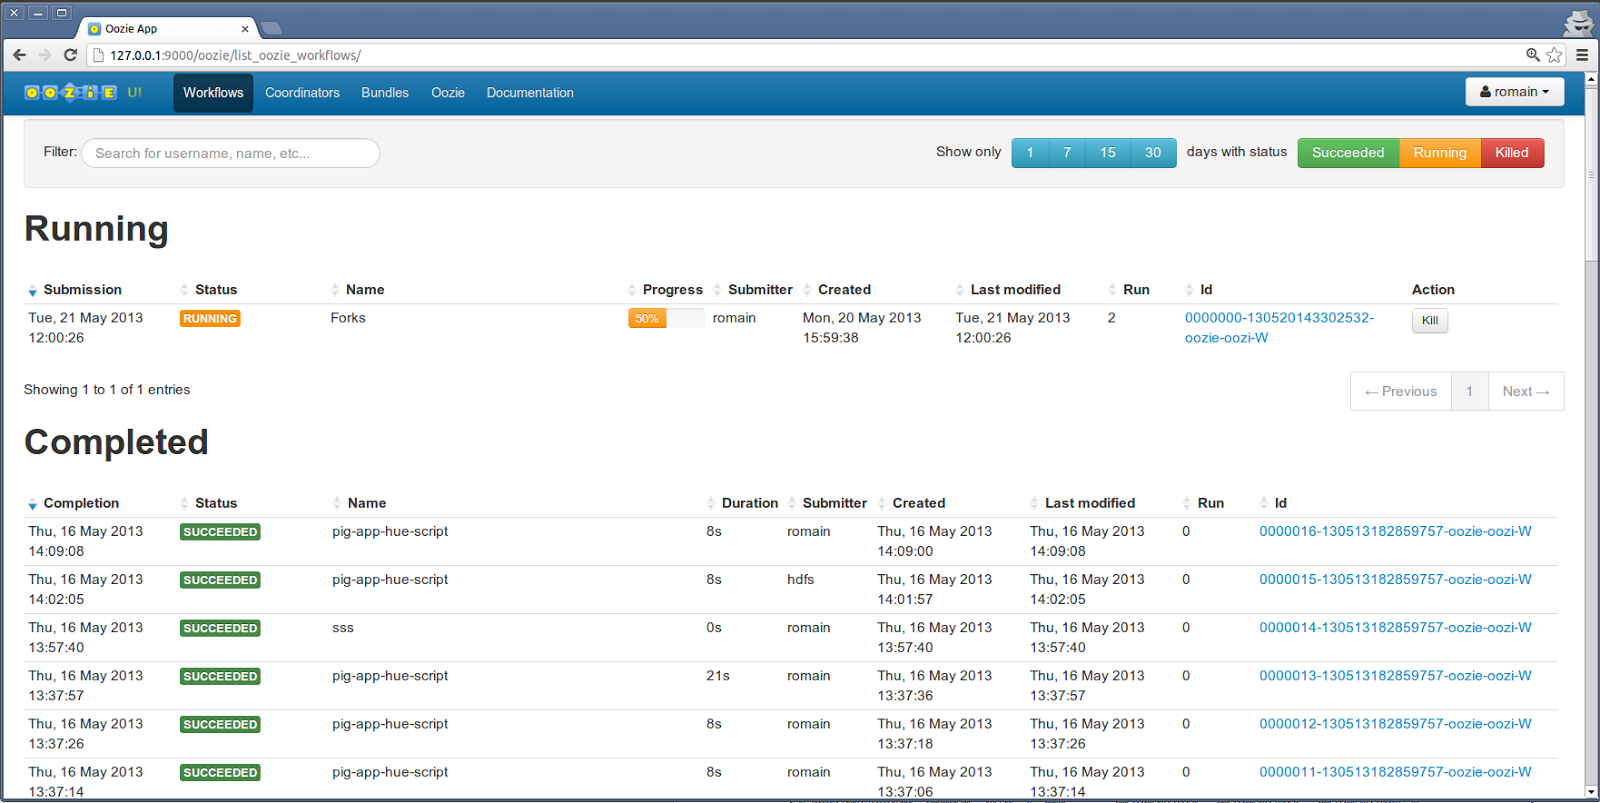
\includegraphics[width=\linewidth]{Imagens/hue-oozie}
%     \caption{Interface com Hue}
%     \label{fig:hue}
% \end{figure*}

% O agendamento de tarefas pode ser feito usando a sintaxe básica do CRON, apesar de não depender desta ferramenta. 
% % estruturado como um grado é possível ter uma visão dos jobs se obtiveram sucesso ou não, em alguns casos é possível visualizar até mesmo ver os logs de execução.

% % mecanismo de execução de \textit{workflow} baseado em servidor, sendo uma ferramenta de código aberto mantido e 
% % Essa ferramenta tem como principal objetivo ser confiável, escalável e extensível para definir, gerenciar, agendar e executar \textit{workflows} complexas do Hadoop por meio de serviços da web, usando um controle de dependências através de um grafo acíclico direcionado. 

% % A execução de um job do Oozie ocorre através da sua inicialização em um sistema remoto(Hadoop, Pig). Após a finalização de um passo, é enviada uma resposta de volta notificando o resultado da ação, a partir dessa resposta o próximo passo do workflow é executado.

% % Para o desenvolvimento de jobs são criados arquivos no formato de um XML baseado no Hadoop Process Definition Language (hPDL) schema. Devido a esse formato, a criação de jobs é mais complexa, dificultando a manutenção e se tornando propenso a cometer erros.

% % A estrutura dos jobs consiste de dois tipos nós: controle de fluxo e ação. Nós de controle de fluxo definem o início e o final de um workflow(Inicialização, finalização e falha de nós) e além disso, providencia um mecanismo para a definição do caminho do workflow(Decisões, divisão  ou junção de nós).Os nós de ação são o mecanismo pelo qual um workflow aciona a execução de uma tarefa de processamento.

% % Para a criação do ambiente são necessários alguns requisitos como Java 8, Unix e Hadoop. A partir destes requisitos, são executados alguns scripts para a configuração e inicialização, fazendo com que o processo seja bem simplificado, caso não haja muitas alterações nas configurações.


% \subsection{Aurora}

% O Aurora é um gerenciador de \textit{workflow} para infraestruturas distribuídas gerenciadas pelo Mesos, ambos da ASF. 
% % que tem como objetivo rodar longos serviços, cron jobs e ad-hoc jobs. Possui código aberto e 
% Apesar da dependência de infraestrutura distribuída (e especificamente do Mesos), é usado por grandes empresas como Uber, Twitter e PayPal. A documentação existente é bastante completa e possui uma comunidade ativa que ajuda tanto no desenvolvimento da ferramenta, como também para dúvidas a respeito do seu uso.

% % O Aurora executa aplicativos e serviços em um conjunto compartilhado de máquinas e é responsável por mantê-los em execução para sempre. Quando as máquinas apresentam falhas, o Aurora reprograma de forma inteligente esses trabalhos em máquinas prontas para uso.

% O Aurora possui uma interface gráfica própria simples contendo as informações referentes aos \textit{jobs}, como tempo de execução e \textit{logs}. 

% Com a utilização do Apache Mesos, é possível ter uma interface gráfica que possa visualizar as principais informações a respeito das operação que ocorreram, além disso existem outras ferramentas que também podem ser utilizadas para se obter uma interface gráfica como Eclipse e Hue.

% \begin{figure}[htp]
%     \centering
%     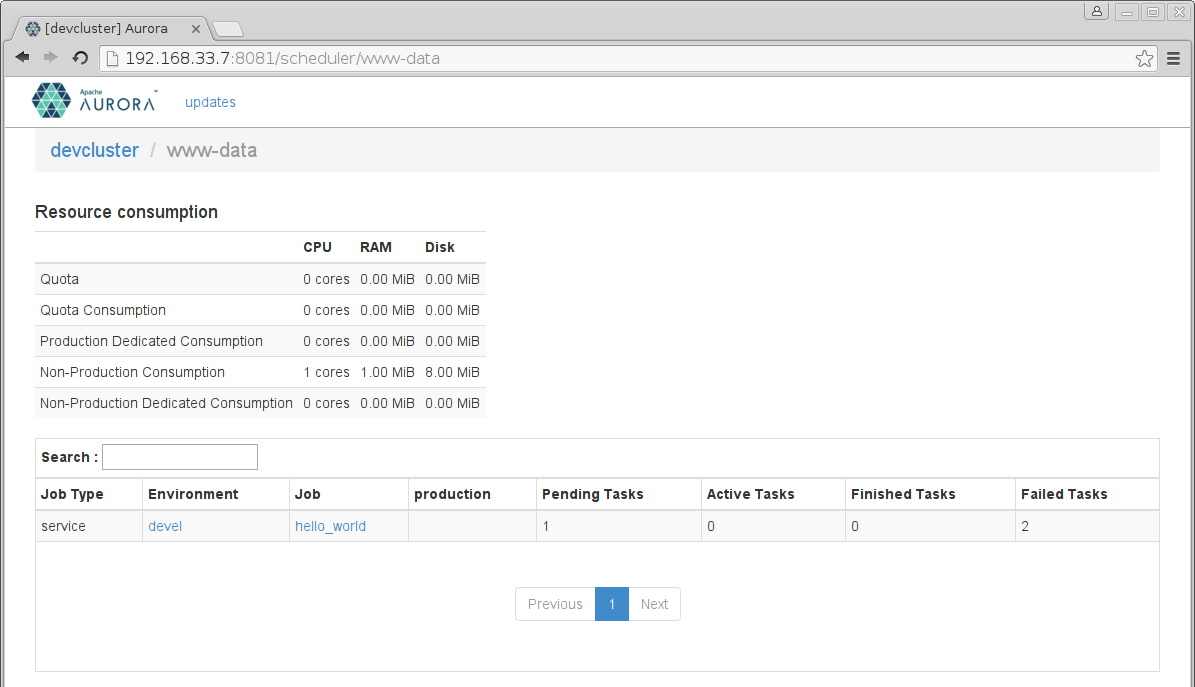
\includegraphics[width=8cm]{Imagens/Aurora_GUI}
%     \caption{Interface Aurora}
%     \label{fig:galaxy}
% \end{figure}

% Para a criação de jobs, é necessário a criação de um arquivo de configuração aurora onde possui o mesmo formato que um arquivo Python, contudo possuindo algumas peculiaridades da sintaxe criada pelo Aurora e caso seja necessário, um outro arquivo contendo as instruções do processo. A partir do arquivo de configuração é possível definir dependências ou até mesmo concorrência entre tarefas. Após a criação dos arquivos, é necessário acessar a máquina virtual em que o Aurora se encontra e executar os comandos necessários para que o job possa ser agendado. Esse processo completo pode acabar dificultando a manutenção dos jobs por não ser tão direto.

% Para entender como o Aurora funciona, precisamos entender o que é o Apache Mesos. Mesos é um projeto de código aberto para gerenciar clusters de computadores, ele abstrai a CPU, a memória, o armazenamento e outros recursos de computação das máquinas (físicas ou virtuais), permitindo que sistemas distribuídos elásticos e tolerantes a falhas sejam facilmente construídos e executados com eficiência.

% Com base nisso, é definida uma arquitetura com o Aurora contendo os componentes que realizam a sua execução. A partir dessa estrutura ocorre o fluxo de execução, onde o aurora scheduler age como a interface principal com o Mesos, passando os comandos que devem ser instruídos para o Mesos Master. Em seguida, o master será o responsável por organizar a forma de distribuição dos comandos para os outros workers no cluster. No worker, o Mesos agent passará os comandos do Master para o aurora executor, onde irá executar o comando desejado. 

% \begin{figure}[htp]
%     \centering
%     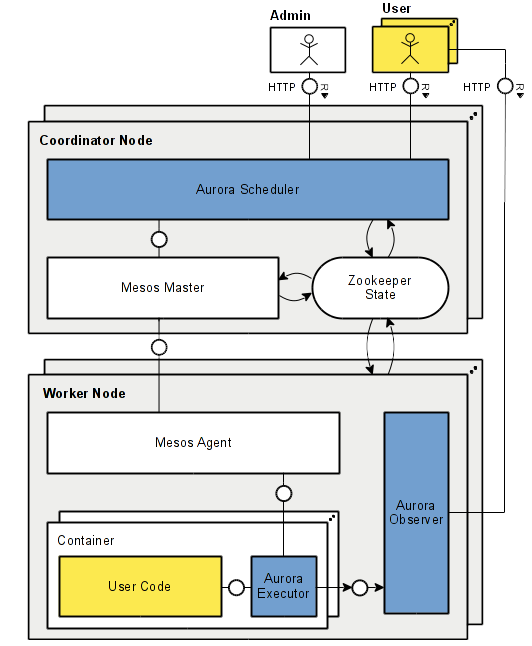
\includegraphics[width=8cm]{Imagens/Aurora_Arch}
%     \caption{Arquitetura Aurora}
%     \label{fig:galaxy}
% \end{figure}

% 	Para a configuração do ambiente, o processo é um pouco grande devido a quantidade de ferramentas que devem ser instaladas por ser necessário a instalação do Apache Mesos, contudo os componentes são de fácil instalação e configuração entre si.
% 	A documentação existente é bastante completa e possui uma comunidade ativa que ajuda tanto no desenvolvimento da ferramenta, como também para dúvidas a respeito do seu uso.

\paragraph{Luigi}
é um pacote Python desenvolvido pelo Spotify para gerenciamento de \textit{workflows}~\cite{batch}. Apesar de compatível com infraestruturas distribuídas, pode ser utilizado no contexto do TRE-RN. É utilizada em grandes empresas como Foursquare e Red Hat~\cite{redhatwebsite}, dispondo de uma vasta comunidade de usuários que ajudam na resolução de dúvidas. A documentação para a usabilidade da ferramenta é bastante robusta, porém por vezes imprecisa~\cite{luigidocs}. 

A Figura~\ref{fig:luigi} mostra a interface gráfica do Luigi, que é de fácil uso e permite a visualização mas não a criação de \textit{workflows}. No entanto, uma vez que a definição de um \textit{workflow} é feita em Python, é possível utilizar bibliotecas Python especializadas em grafos. Uma vez criado o DAG, o agendamento de sua execução deve ser feita por linha de comando, usando o agendador próprio do Luigi. 
% Além de um agendador local para máquinas de desenvolvimento, o Luigi mantém um agendador central próprio no servidor de produção. 
O \textit{log} de execução de um \textit{workflow} é limitado, informando apenas seu sucesso ou falha.

\begin{figure*}[!t]
    \centering
    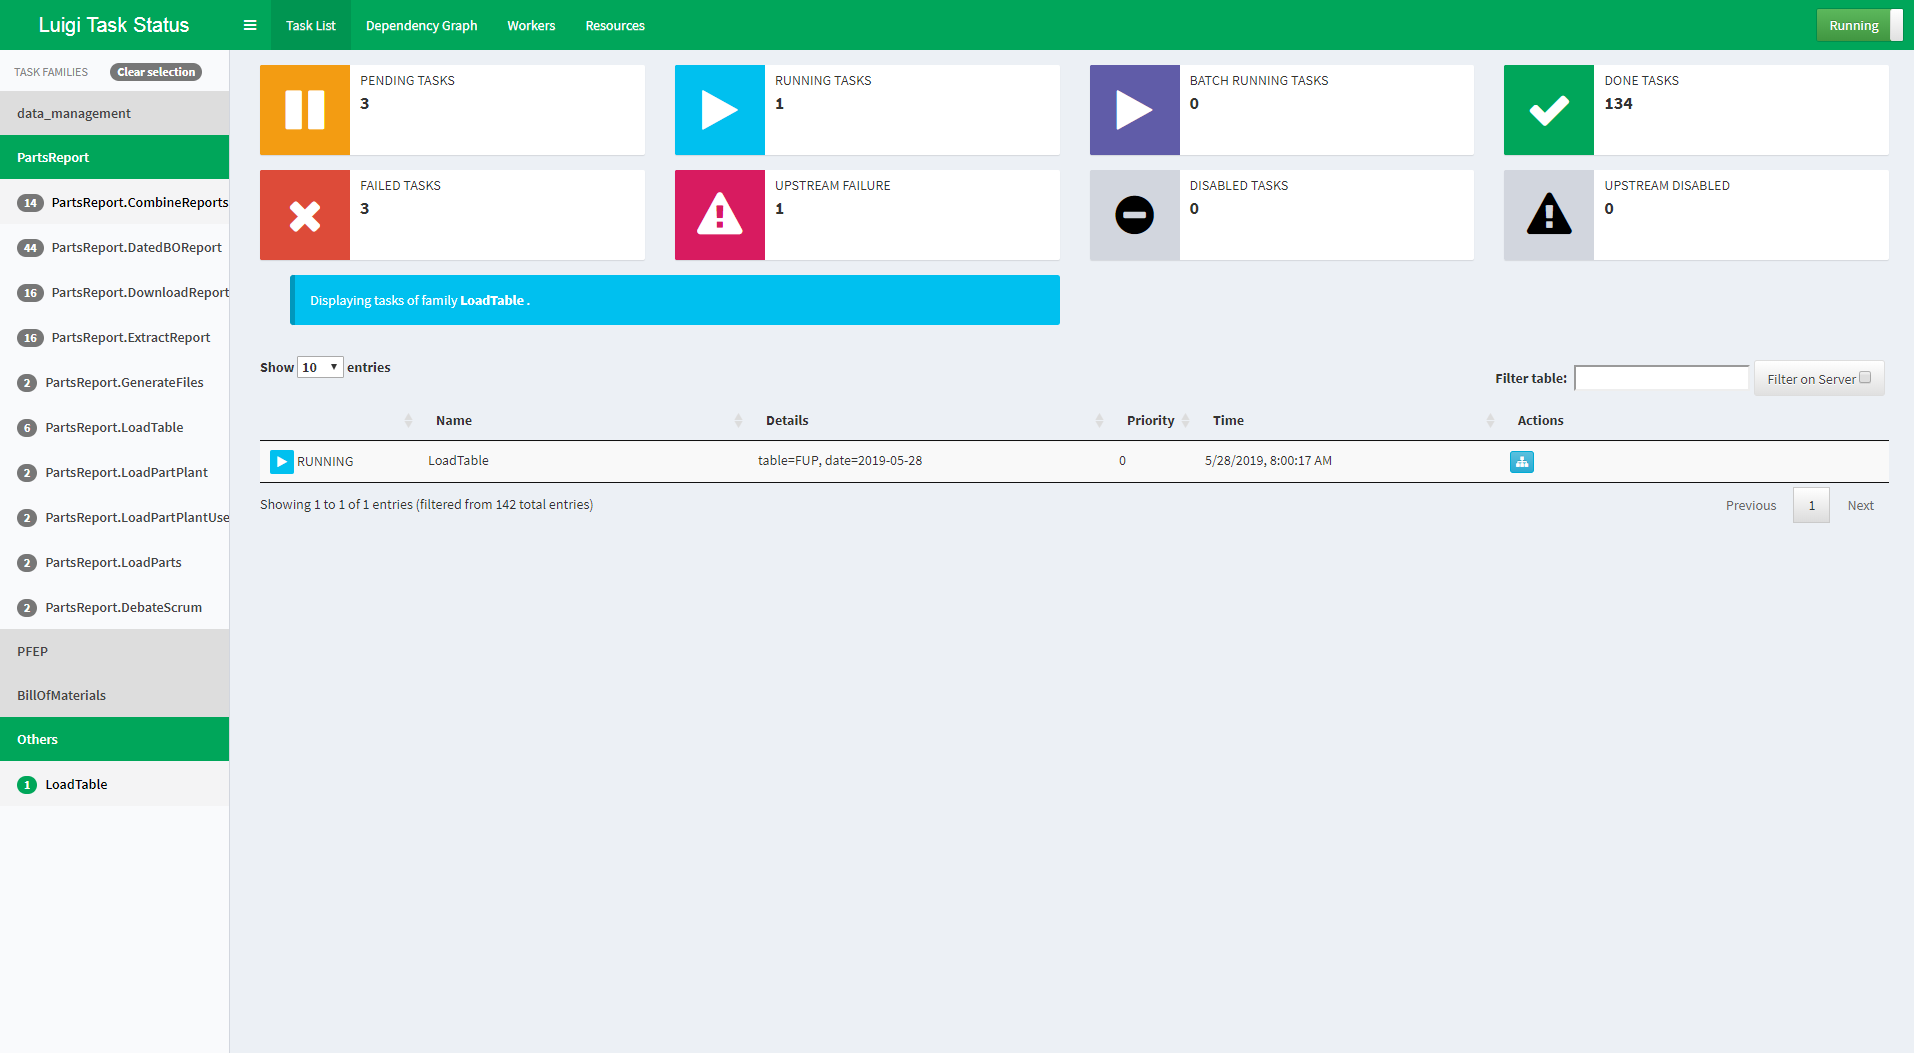
\includegraphics[width=\linewidth, clip=true, trim=0 400px 0 0]{Imagens/Luigi_GUI}
    \caption{Interface do gerenciador de \textit{workflows} \textit{Luigi}.}
    \label{fig:luigi}
\end{figure*}

% A proposta do Luigi é endereçar todas as partes do processo de carregamento de dados em grandes pacotes de classe Python. Essas partes podem ser qualquer coisa, mas os principais usos são com longos jobs Hadoop, descarregamento dados de/para bancos de dados e execução algoritmos de aprendizado de máquina.


% O servidor do Luigi já vem com uma interface web onde é possível ter uma panorama geral dos jobs que já foram executados, além realizar pesquisas e filtragens a respeito desses jobs. 

% O processo de criação de um job no Luigi é feito através do desenvolvimento de um ou mais arquivos Python utilizando dois tipos de classes diferentes: Target e Task.

% \begin{itemize}
% \item Target é a classe utilizada no Luigi com o objetivo realizar a checagem referente a algum tipo de entrada, essa entrada pode ser um arquivo de disco, arquivo HDFS ou um banco de dados. Uma classe simples que serve ponto inicial do ETL.
% \item Task é a classe onde ocorre o processamento. Nessa classe existem alguns métodos que podem ser implementados para mudar seu comportamento, mais notavelmente os métodos run, requires e output.
% \begin{itemize}
% \item Run é o método da classe em que a lógica de processamento ocorre.
% \item Requires é o método utilizado para a definição da dependências entre Tasks.
% \item Output tem como objetivo gerar uma saída dessa classe.
% \end{itemize}
% \end{itemize}

% Após a criação dos arquivos, é necessário que as transformações sejam executadas através de linha de comando na máquina onde o Luigi se encontra.
% O aspecto mais importante é que nenhuma execução é transferida. 
% Quando você executa um workflow do Luigi, o worker agenda todas as tarefas e também executa as tarefas no processo.

% \begin{figure}[htp]
%     \centering
%     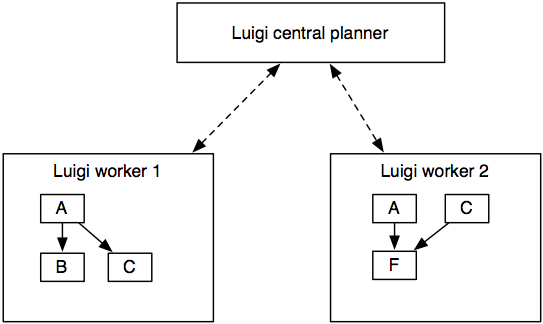
\includegraphics[width=7cm]{Imagens/execution_model}
%     \caption{Arquitetura Luigi}
%     \label{fig:galaxy}
% \end{figure}

% Apesar de possuir uma interface gráfica de fácil usabilidade, a forma como se cria os arquivos para a criação de job com o uso um paradigma diferente através das tasks e targets, torna o processo um pouco complicado. Além disso, o Luigi não possui um scheduler próprio, sendo necessário o uso do Cron para o agendamento dos jobs, com isso fica difícil dar manutenção aos jobs existentes.

% A configuração do ambiente é simples, sendo necessário apenas subir o servidor com a interface do luigi e um banco de dados para o armazenamento dos metadados de cada job que ocorreu.

% A documentação para a usabilidade da ferramenta é bastante robusta e volumosa, contudo existem algumas partes que as explicações são um pouco confusas, dificultando o entendimento de certas coisas. Por ser uma das ferramentas mais usadas no mercado, existe uma vasta comunidade de usuários que ajudam na resolução de dúvidas.


\paragraph{Azkaban}
é um gerenciador de \textit{workflows} desenvolvido pelo LinkedIn para gerenciar processos de ETL em ambientes Hadoop~\cite{}. Apesar de compatível com infraestruturas distribuídas, pode ser utilizado no contexto do TRE-RN. Microsoft e Disney Studios são alguns de seus usuários, dispondo também de uma comunidade ativa. Sua documentação é completa, porém está em processo de reformulação~\cite{azakbandocsnew}.

A Figura~\ref{fig:azkaban} mostra sua interface gráfica, que oferece diversas operações de gerenciamento de \textit{workflows}. A definição de um \textit{workflow} é feita através de arquivos YAML, sendo 
% , isolando a definição do DAG dos códigos a serem executados.
possível agrupar múltiplos \textit{workflows} em um projeto. O agendamento da execução de um \textit{workflow} utiliza um agendador próprio, também configurável através da interface gráfica. Além de informar sobre o sucesso ou falha da execução de um \textit{workflow}, os \textit{logs} disponibilizados pelo Azkaban incluem as mensagens produzidas durante a execução do \textit{workflow}.
Por fim, a interface do \textit{Azkaban} permite visualizar informações a respeito dos metadados de cada \textit{workflow}, como seu desempenho. 

\begin{figure*}[!t]
    \centering
    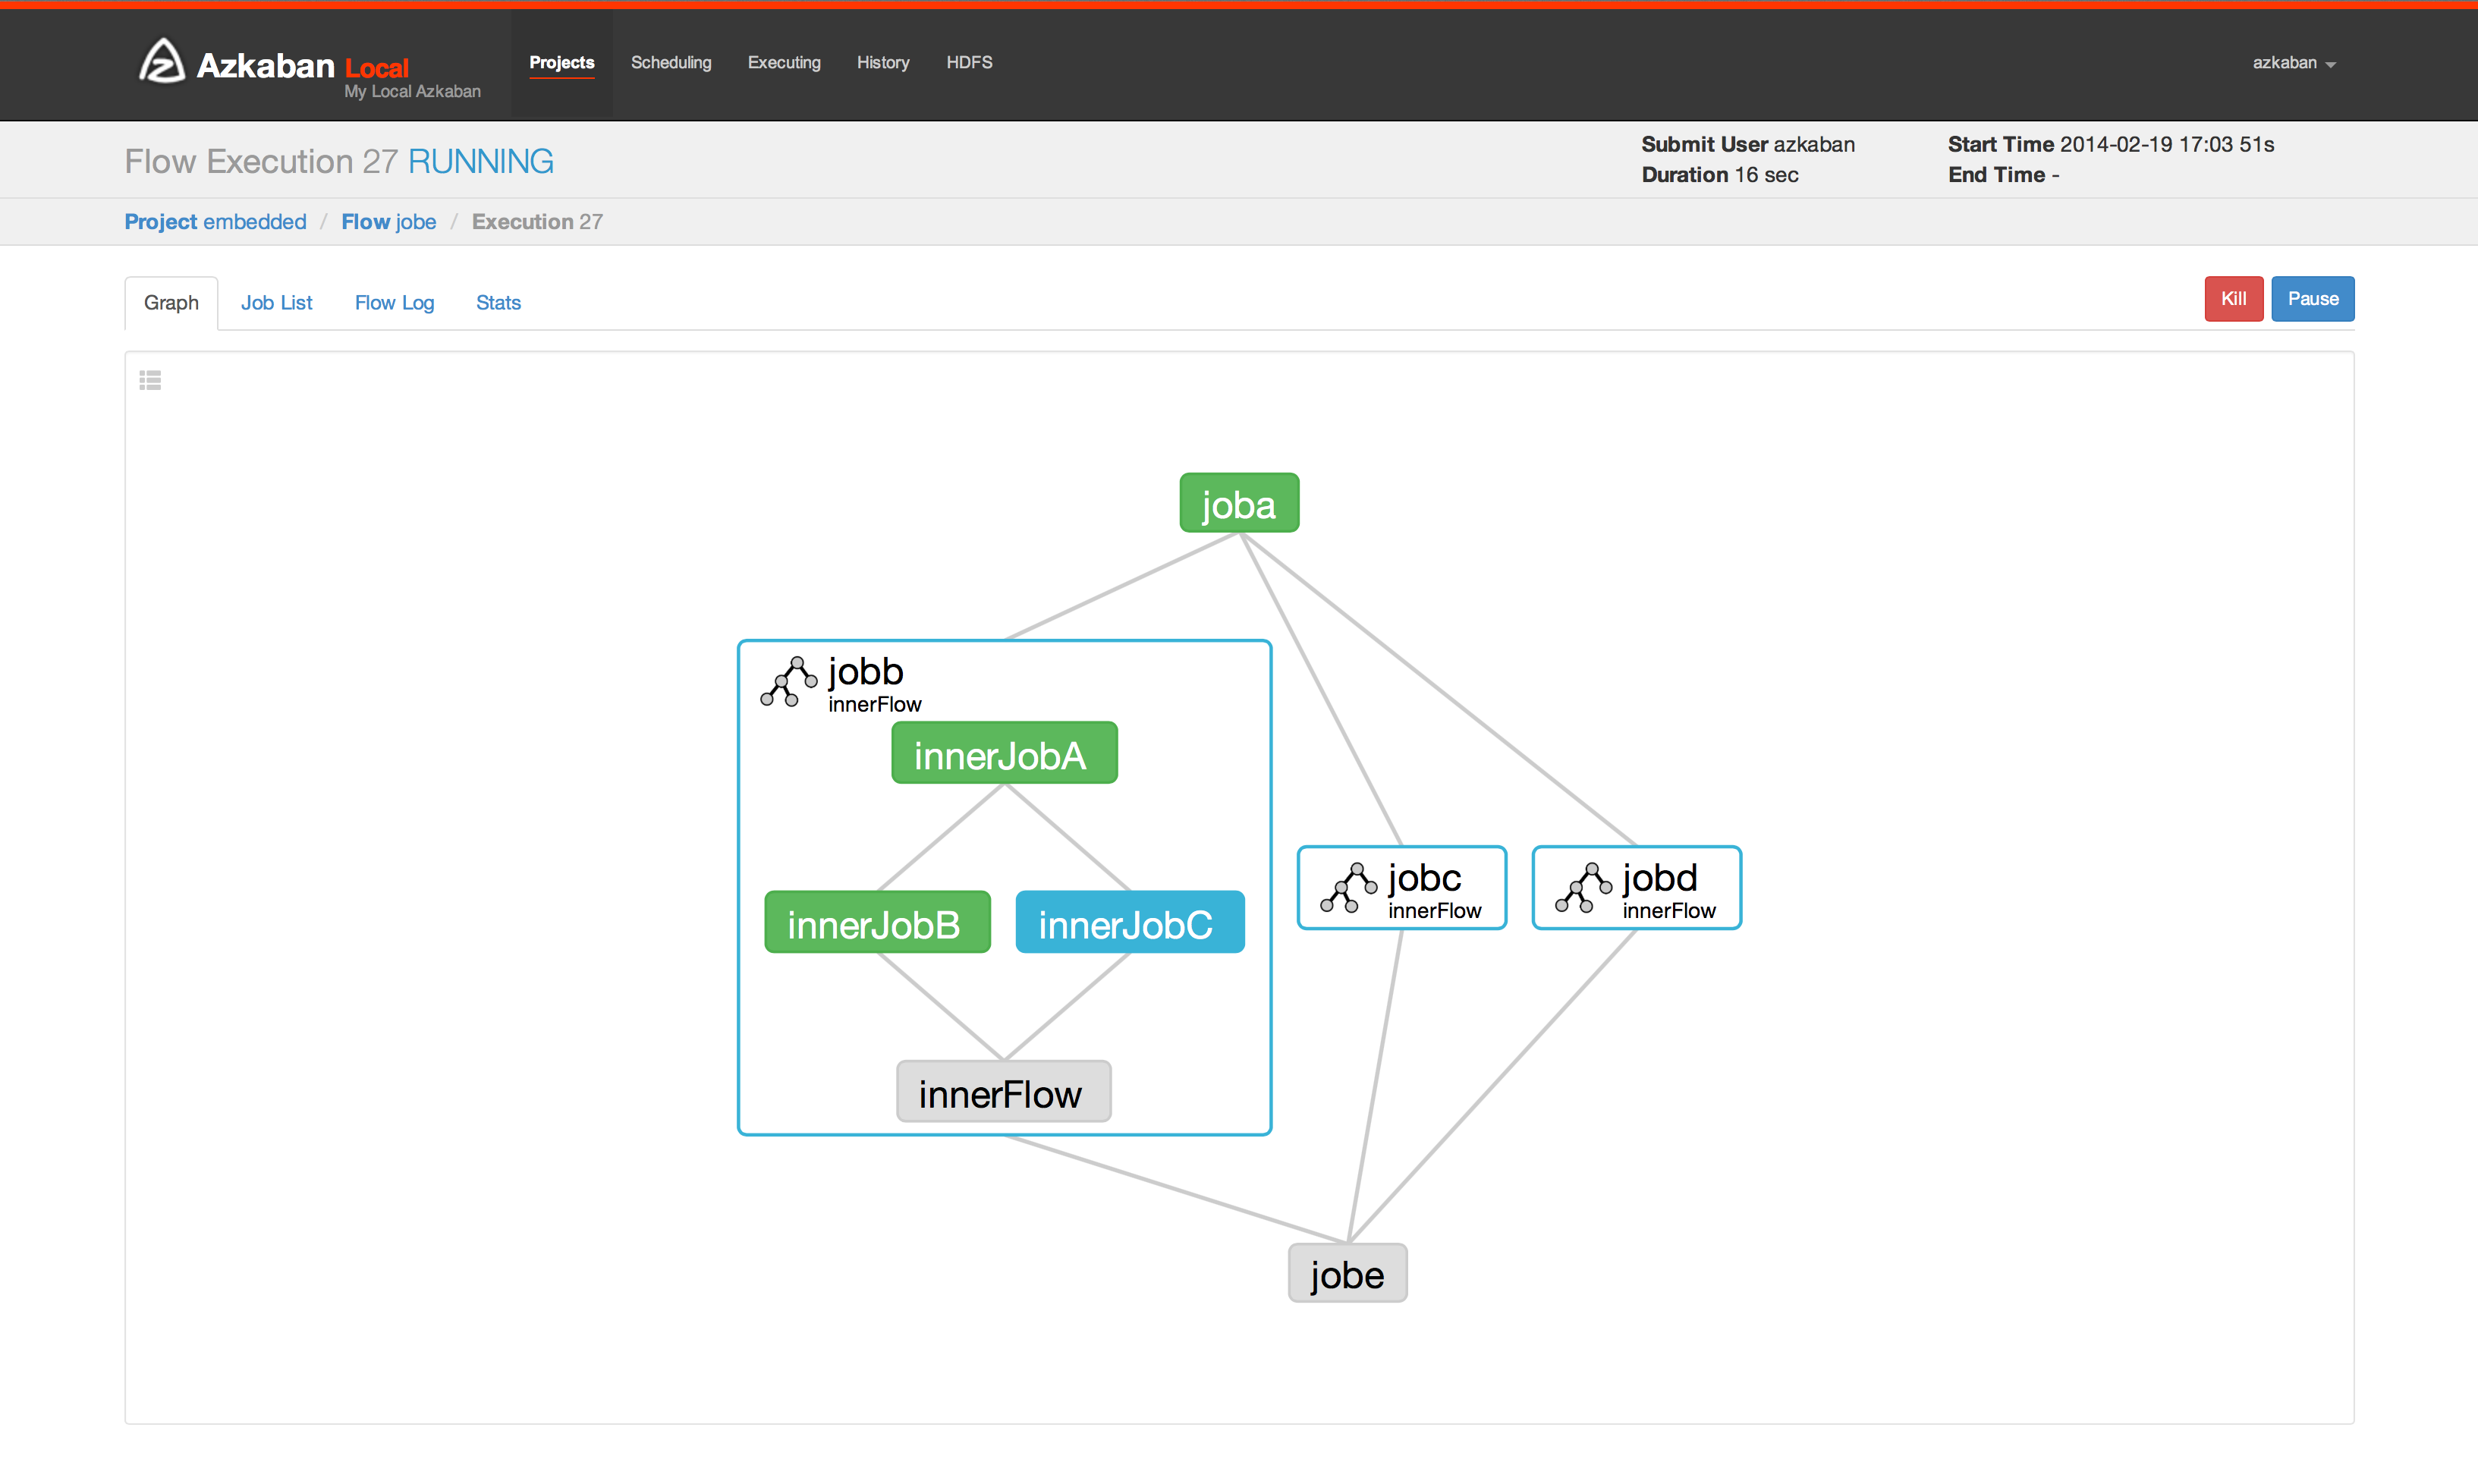
\includegraphics[width=\linewidth, clip=true, trim=0 180px 0 82px]{Imagens/Azkaban_GUI}
    \caption{Interface do gerenciador de \textit{workflows} \textit{Azkaban}.}
    \label{fig:azkaban}
\end{figure*}


% A ferramenta foi desenvolvida com o propósito de realizar o agendamento entre jobs do Hadoop usando uma abordagem de dependência entre jobs, junto com uma interface gráfica que fosse possível acompanhar e manter seus fluxos .Com o aperfeiçoamento da ferramenta, hoje ela também tem como foco o gerenciamento de fluxos de ELT, Spark, aprendizado máquina e até transmissão de dados em tempo real.


% podendo ser feita  ode ser feita 
% É possível criar projetos onde serão definidos os ETL’s, como também fazer o gerenciamento desses projetos. Uma peculiaridade dessa interface é o fato de você fazer o upload dos arquivos a serem usados, a partir da interface, o que deixa o processo mais simples. Além disso, consegue gerar informações a respeito dos metadados de cada ETL, podendo ter informações referentes ao desempenho e aos logs.

% Para a criação de um job, são necessários dois arquivos YAML, um arquivo project e outro arquivo job. O arquivo project tem como objetivo definir a versão da linguagem usada no segundo job. O arquivo job tem como objetivo definir o ETL, nesse arquivos são definidos nós(um comando), o fluxo entre esse nós e propriedades referentes a essa transformação. Além disso, é possível usar mais de um arquivo job para a definição do ETL, facilitando a organização e manutenção da ferramenta. 

% A estrutura do Azkaban é pode ser feita de duas formas: Single Server ou Multi Server. Na primeira abordagem, um único servidor realiza todas as funcionalidades e é usado um banco H2 para armazenamento dos metadados. Na segunda abordagem, o Azkaban é dividido em três partes: banco de dados relacional, Azkaban Web Server e Azkaban ExecutorServer. O banco de dados relacional tem como objetivo guardar os metadados e o estado do Azkaban. O Azkaban Web Server é gerenciador principal de todo o Azkaban, além de ser a interface web, ele tem como objetivo gerenciar os projetos, a autenticação, o agendador e fazer o monitoramento das execuções. O Azkaban ExecutorServer é onde ocorre a execução dos jobs, por ser separado do Web Server, é possível escalar a quantidade de Executors, tornando-se possível a distribuição de jobs e a alta disponibilidade, caso um Executor falhe. 

% \begin{figure}[htp]
%     \centering
%     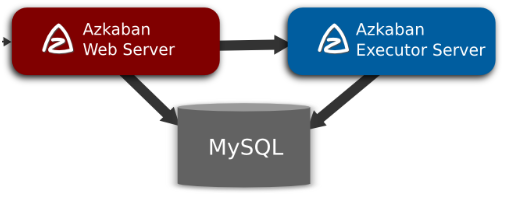
\includegraphics[width=8cm]{Imagens/Azkaban_Arc}
%     \caption{Arquitetura Azkaban}
%     \label{fig:galaxy}
% \end{figure}

% A criação do ambiente com Azkaban é bastante simples, tanto para o Single Server como para o Multi Server. A maior dificuldade se encontra no Multi Server por ser necessário levantar pelo menos três aplicações, contudo ainda é relativamente simples.
% Possui uma comunidade bastante ativa, além de uma documentação muito completa, onde é possível aprender todas as informações necessárias para levantar a aplicação, entender seu funcionamento e iniciar o desenvolvimento a usando.

\paragraph{Airflow}
é uma ferramenta originalmente desenvolvida pela Airbnb e atualmente mantida pela ASF~\cite{apache}. É utilizada por empresas como Adobe e Ubisoft. Apesar de ser a ferramenta-padrão na Google Cloud Platform, não se aplica apenas a ambientes distribuídos, podendo ser utilizada no contexto do TRE-RN. Por ser uma das ferramentas mais populares, dispõe de uma grande comunidade para suporte, como também uma documentação muito completa rica em exemplos~\cite{airflowdocs}.

A Figura~\ref{fig:airflow} ilustra a interface gráfica do Airflow. Assim como no Azkaban, é possível detalhar cada \textit{workflow} quanto a dependências, desempenho e \textit{log} de execução. A criação de um \textit{workflow} é feita em Python, como no \textit{Luigi}, e seu agendamento é discriminado em um arquivo de configuração específico do \textit{workflow}. É possível visualizar o código-fonte do \textit{workflow} e gerenciar sua execução iterativamente, forçando sua execução imediata ou (des)ativando seu agendamento. O \textit{log} de execução inclui todas as mensagens produzidas pelo \textit{workflow}, assim como no Azkaban.

\begin{figure*}[!t]
    \centering
    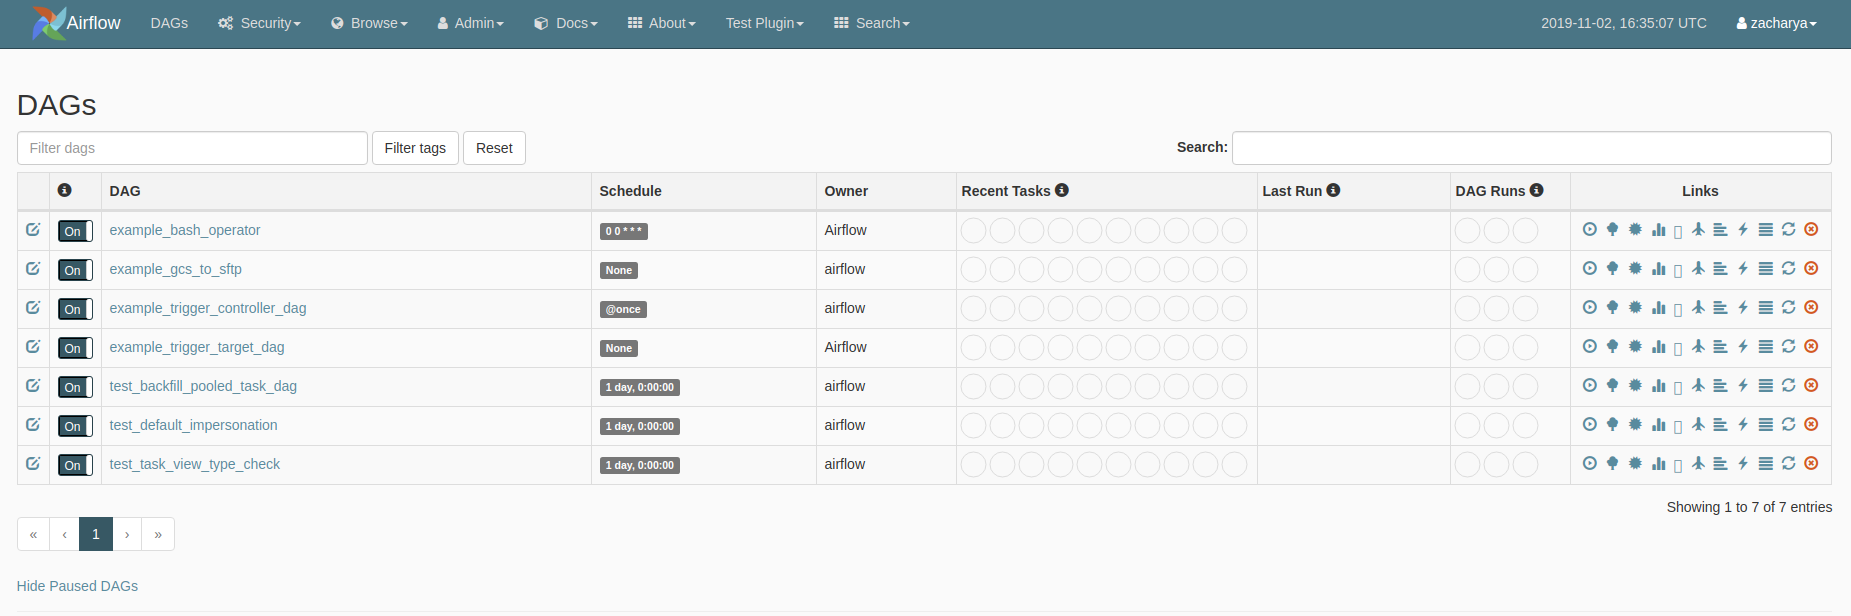
\includegraphics[width=\linewidth]{Imagens/dags}
    \caption{Interface do gerenciador de \textit{workflow} \textit{Airflow}.}
    \label{fig:airflow}
\end{figure*}


% Por ser uma das ferramentas mais populares, , entre outras.
% Tem como objetivo criar, programar e monitorar programaticamente \textit{workflows} usando os seguintes princípios:

% \begin{itemize}
% \item Escalável - Com o uso de uma arquitetura modular e uma fila de mensagens, é possível orquestrar uma quantidade de worker desejáveis
% \item Dinâmico - As configurações do pipeline são feitas em código permitindo uma geração dinâmica do pipeline. Isso permite escrever código que instancia pipelines dinamicamente.
% \item Extensível - Definição de seus próprios operadores, executores, fazendo com que  se estenda a biblioteca para que ela se ajuste ao nível de abstração que se adapte ao ambiente do usuário.
% \item Elegante - Os pipeline são de fácil entendimento e explícitos.
% \end{itemize}

% O airflow possui uma interface gráfica bastante robusta e interativa. Nela é possível ver todas as informações referentes a cada job como desempenho, dependências, log e código. Além disso, a interface também é usada para interagir, podendo forçar inicialização ou ligar/desligar qualquer job. 

% A criação de um job é feita através de um código em python utilizando os conceitos de Directed acyclic graph(DAG), operator e task. Um operator é Uma classe que atua como modelo para realizar algum trabalho, como a execução de um script em bash. A task é uma instância que define valores específicos ao se chamar um operador no qual se torna um nó na DAG. Através de um script python a DAG é definida como uma coleção de todas as tasks que você deseja executar, organizadas de maneira a refletir seus relacionamentos e dependências. Após o processo de criação, os arquivos criados devem ser colocados na pasta no qual o Airflow fica observando, após um tempo determinado pela ferramenta, a DAG aparece na interface gráfica disponível para o uso.

% A arquitetura do Airflow pode ser feita de duas formas: arquitetura de um nó ou arquitetura de múltiplos nós. A arquitetura de um nó é definida através das seguintes estruturas:

% \begin{itemize}
% \item Webserver - É o responsável por abrir a interface do navegador e mostrar os metadados das DAG’s e tasks.
% \item Scheduler - Verifica o status das DAGs e tasks no banco de dados de metadados, cria novos, se necessário, e envia as tarefas para as filas.
% \item LocalExecutor - Empurra as tasks agendadas na fila.
% \item Airflow Worker - recupera os comandos das filas, os executa e atualiza os metadados.
% \end{itemize}

% A arquitetura de múltiplos nós possui todas as estruturas da arquitetura de um nó, com a adição de múltiplos Airflow Workers e um Queuing service para realizar a orquestração da fila de comandos para os workers.

% \begin{figure}[htp]
%     \centering
%     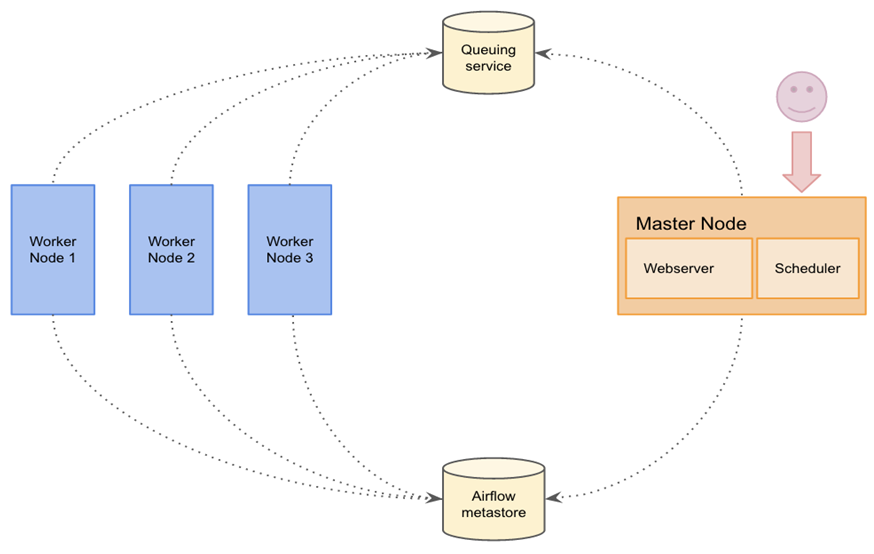
\includegraphics[width=8cm]{Imagens/image-26}
%     \caption{Arquitetura Airflow}
%     \label{fig:galaxy}
% \end{figure}

% Por ter uma interface bastante robusta com foco em lean, a ferramenta se torna bastante fácil se ser usada. Além disso, por ser apenas colocar o script python na pasta selecionada para leitura, facilita a execução e manutenção da ferramenta.

% A complexidade da configuração do ambiente varia de acordo com a arquitetura. A arquitetura de um nó é mais simples por conter apenas um nó, contudo na arquitetura de múltiplos a configuração se torna mais complexa por precisar de um Queuing service para orquestrar vários workers.

% Por ser uma das ferramentas mais populares de gerenciamento de workflow, existe uma grande comunidade para dar suporte, como também possui uma documentação muito completa com muitos exemplos.

\subsection{Discussão}

A análise acima mostra que apenas o Airflow atende completamente a todos os critérios de adequação ao contexto do TRE-RN. Adicionalmente, seria possível considerar também as ferramentas \textit{Luigi} e \textit{Azkaban}, porém cada uma traz algum tipo de limitação significativa. Especificamente, pesam contra o \textit{Luigi} sua interface gráfica e a dependência de linha de comando para o agendamento de tarefas. No caso do Azkaban, a documentação em processo de reformulação e a definição de \textit{workflows} usando YAML são aspectos indesejáveis. Na próxima seção, detalhamos a aplicação do Airflow ao gerenciamento de \textit{workflows} no TRE-RN.

% das ferramentas que apresentadas, decidimos usar o Airflow por ser a ferramenta que mais se encaixa nos critérios de seleção. Com base nisso, explicamos sua seleção em cada critério.

% \textbf{Adequação a infraestrutura}: Por possuir uma estrutura centralizada em uma aplicação única, sua implantanção acaba sendo mais fácil de ser implantada e de realizar manutenção.

% \textbf{Disseminação e suporte}: Com uma grande quantidade de empresas que usam o Airflow, a ferramenta possui uma vasta comunidade de usuários que ajudam na resolução de dúvidas.

% \textbf{Documentação}: Além de possuir uma documentação bastatne extensa e completa, a ferramenta também contém uma grande quantidade de exemplos, facilitando no aprendizado de uso.

% \textbf{Interface gráfica}: Possui uma interface gráfica bastante completa, fácil de ser usada e interativa que permitir realizar as pricipais operações no gerenciamento de um \textit{workflow}. Além disso, o Airlfow permite a amplicação da prórpia interface gráfica através de criação de páginas pelo próprio usuário.

% \textbf{Criação de \textit{workflows}}: Por ter uma curva de aprendizado pequeno, a criação de \textit{workflows} se torna fácil e intuitiva. Além disso, o Airflow possui suporte para diversos tipos de operações que facilitam no processo de desenvolvimento de um \textit{workflow}, como conexão SSH, conexão a bancos de dados, entre outras operações.

% \textbf{Agendamento}: Por ter um agendador próprio, o Airflow não fica dependente de agendadores externos, fazendo com que o processo fique todo centralizado na ferramenta.

% \textbf{Log de Execução}: O Airflow consegue exibir o log das transformações executadas de uma maneira fácil, o que ajuda no processo de debug dos \textit{jobs}.

% Apesar do Luigi ser uma ferramenta possível de ser aplicada no TRE-RN, alguns fatores influenciaram para que não o escolhêssemos escolhido. Os fatores que influenciaram foram:

% \textbf{Interface gráfica}: A interface gráfica da ferramenta é limitada, sua função é apenas exibir algumas informações a respeito dos jobs, não sendo interativo.

% \textbf{Documentação}: Apesar de ter uma documentação bastante robusta, em certas partes os conceitos não são explicados de uma forma muito clara. 

% \textbf{Criação de \textit{workflows}}: Agregado com a documentação não ser muito clara em certos aspectos, a criação dos \textit{workflows} usam uma estrutura com uma curva de aprendizado alta que dificulta a criação de \textit{workflows}.

% \textbf{Agendamento}: A ferramenta não possui um agendador próprio, fazendo com seja necessário programas externos para que o agendamento de jobs seja realizado.

% Assim como o Luigi, o Azkaban também é uma ferramenta que poderia ser utilizada no TRE-RN, mas diante de alguns fatores, ele não o escolhido. Esses fatores foram:

% \textbf{Documentação}: Apesar de possuir um documentação completa, ela está em processo de reformulação.

% \textbf{Criação de \textit{workflows}}: Por não usar uma linguagem de programação para usos gerais, a capacidade de criação de workflows da ferramenta acaba de tornando limitada.

% Apesar destas duas ferramentas não terem sido selecionadas para o contexto atual, ambas podem ser consideradas viáveis, em algum contexto futuro em que algum tipo de mudança arquitetural seja feita no que existe altualmente. 